%% thesis.tex 2014/04/11
%
% Based on sample files of unknown authorship.
%
% The Current Maintainer of this work is Paul Vojta.
%
% https://math.berkeley.edu/~vojta/tex/ucbthesis-phd.html

\documentclass{ucbthesis}
\usepackage[dvipdfmx]{graphicx} % needs to be up top
\usepackage{bmpsize}
\usepackage{blkarray}
\usepackage{amsmath}
\usepackage{amssymb}
\usepackage{color}
\usepackage[super]{nth}
\usepackage{tikz}
\usepackage{tikz-3dplot}
\usetikzlibrary{arrows}
\usetikzlibrary{decorations.pathreplacing, decorations.markings}
\usetikzlibrary{3d,angles,quotes,calc,shapes}
\usetikzlibrary{shapes.geometric}
\usetikzlibrary{positioning}
\usepackage[export]{adjustbox} % must be below tikz else tikzplots are scronched
\usepackage[version=3]{mhchem}
\usepackage{multirow}
\usepackage{subcaption}
\usepackage{pst-all}


%For inclusion of figures
\usepackage{graphicx}

\tikzstyle{startstop} = [rectangle, rounded corners, minimum width=3cm, minimum height=1.0cm, text centered, draw=black, fill=lightgray]
\tikzstyle{process} = [rectangle, minimum width=6cm, minimum height=1.0cm, text width = 5cm, text centered, draw=black, fill=lightgray]
\tikzstyle{decision} = [diamond, minimum width=2cm, minimum height=1cm, text width = 3cm, text centered, draw=black, fill=lightgray]
\tikzstyle{io} = [trapezium, trapezium left angle=70, trapezium right angle=110, minimum width=3cm, text width = 3cm, minimum height=1cm, text centered, draw=black, fill=lightgray]
\tikzstyle{arrow} = [thick,->,>=stealth]
\tikzstyle{vecArrow} = [thick, decoration={markings,mark=at position
   1 with {\arrow[semithick]{open triangle 60}}},
   double distance=1.4pt, shorten >= 5.5pt,
   preaction = {decorate},
   postaction = {draw,line width=1.4pt, white,shorten >= 4.5pt}]
\tikzstyle{innerWhite} = [semithick, white,line width=1.4pt, shorten >= 4.5pt]

\newcommand{\CommonElementTextFormat}[4]
{
  \begin{minipage}{2.2cm}
    \centering
      {\textbf{#1} \hfill #2}%
      \linebreak \linebreak
      {\textbf{#3}}%
      \linebreak \linebreak
      {{#4}}
  \end{minipage}
}

\newcommand{\NaturalElementTextFormat}[4]
{
  \CommonElementTextFormat{#1}{#2}{\LARGE {#3}}{#4}
}

\newcommand{\OutlineText}[1]
{
\ifpdf
  % Couldn't find a nicer way of doing an outline font with TikZ
  % other than using pdfliteral 1 Tr
  %
  \pdfliteral direct {0.5 w 1 Tr}{#1}%
  \pdfliteral direct {1 w 0 Tr}%
\else
  % pstricks can do this with \pscharpath from pstricks
  %
  \pscharpath[shadow=false,
    fillstyle=solid,
    fillcolor=white,
    linestyle=solid,
    linecolor=black,
    linewidth=.2pt]{#1} 
\fi
}

\newcommand{\SyntheticElementTextFormat}[4]
{
\ifpdf
  \CommonElementTextFormat{#1}{#2}{\OutlineText{\LARGE #3}}{#4}
\else
  % pstricks approach results in slightly larger box
  % that doesn't break, so fudge here
  \CommonElementTextFormat{#1}{#2}{\OutlineText{\Large #3}}{#4}
\fi
}

% To compile this file, run "latex thesis", then "biber thesis"
% (or "bibtex thesis", if the output from latex asks for that instead),
% and then "latex thesis" (without the quotes in each case).

% Double spacing, if you want it.  Do not use for the final copy.
% \def\dsp{\def\baselinestretch{2.0}\large\normalsize}
% \dsp

% If the Grad. Division insists that the first paragraph of a section
% be indented (like the others), then include this line:
% \usepackage{indentfirst}

\newtheorem{theorem}{Jibberish}

\hyphenation{ADDER}

\begin{document}

% Declarations for Front Matter

\title{Predicting Fuel Salt Composition via Linear Optimization in Molten Salt
Reactors}
\author{Daniel D. Wooten}
\degreesemester{Fall}
\degreeyear{2019}
\degree{Doctor of Philosophy}
\chair{Assistant Professor Massamiliano Fratoni}
\othermembers{
	Associate Professor Per-Olof Persson \\
	Professor Jasmina Vuji\'c \\
	Dr. Steven P. Hamilton
	}
\numberofmembers{4}
\field{Engineering -- Nuclear Engineering}
% Designated Emphasis -- this is optional, and rare
\emphasis{Computational and Data Science and Engineering}
\campus{Berkeley}

\maketitle
% Delete (or comment out) the \approvalpage line for the final version.
% \approvalpage
\copyrightpage

% (This file is included by thesis.tex; you do not latex it by itself.)

\begin{abstract}

This is blank

\end{abstract}


\begin{frontmatter}

% You can delete the \clearpage lines if you don't want these to start on
% separate pages.

\setcounter{secnumdepth}{3}
\setcounter{tocdepth}{3}

% to show paragraphs in ToC (good for an outline, stylistically ugly):
% \setcounter{secnumdepth}{4}
% \setcounter{tocdepth}{4}

\tableofcontents
\clearpage
\listoffigures
\clearpage
\listoftables

\begin{acknowledgements}
\small

\scriptsize{This material is based upon work supported under an Integrated
University Program Graduate Fellowship as well as supported by the Department 
of Energy under Award Number(s) DE-NEXXXXXX. 
This material is based upon work supported under a Nuclear Regulatory 
Commission Fellowship under Award Number(s) DE-NEXXXXXX. 
This material is based upon work supported under a Nuclear Science and Security 
Cosortium Fellowship under Award Number(s) DE-NEXXXXXX. 
This report was prepared as an account  of work sponsored by an agency of the 
United States Government. Neither the United 
States Government nor any agency thereof, nor any of their employees, makes any 
warranty, express or limited, or assumes any legal liability or responsibility for the 
accuracy, completeness, or usefulness of any information, apparatus, product, or
process disclosed, or represents that its use would not infringe privately owned
rights. Reference herein to any specific commercial product, process, or service by
trade name, trademark, manufacturer, or otherwise does not necessarily constitute or
imply its endorsement, recommendation, or favoring by the United States Government or
any agency thereof. The views and opinions of authors expressed herein do not 
necessarily state or reflect those of the United States Government or any agency 
thereof. This research used the Savio computational cluster resource provided by the 
Berkeley Research Computing program at the University of California, Berkeley 
(supported by the UC Berkeley Chancellor, Vice Chancellor for Research, and Chief 
Information Officer).}

\end{acknowledgements}

\end{frontmatter}

\pagestyle{headings}

% (Optional) \part{First Part}

\chapter{Introduction}\label{ch:intro}

Molten salt reactors (MSRs) first gained attention in the 1950s as a possible
high power density propulsion source for a nuclear powered aircraft. While this
idea never took flight, the possibility for molten salts as fuel for a
nuclear reactor did in the form of the Molten Salt Reactor Experiment (MSRE)
conducted at Oak Ridge National Laboratory (ORNL) during the 1960s and 70s 
\cite{ORNL}. Following an institutional redirection away from the MSRE
program, molten salt studies continued at ORNL under the Molten Salt Breeder
Reactor program through the 1970s and into the 80s \cite{ORNL}. After a
brief lull in global interest during the late 80s and early 90s studies in MSRs
began again in earnest in Europe beginning with the SAMOFAR program and continuing
today under the ALISIA program \cite{SAMOFAR}. Since this time global interest
in MSRs has continued to grow with concepts coming from all corners of the
globe from both industry and governments: the Molten Salt Actinide Recycler and
Transmuter (MOSART) out of Russia, the FUJI series of reactors from Japan, 
the Liquid Fueled Thorium Molten Salt Reactor (LF-TMSR)  out of China, the
Molten Salt Fast Chloride Reactor (MCFR) from TerraPower in the United States,
and many others. While global attention and efforts have also increased around
a group of reactors which use molten salts without fissile content as a coolant,
the fuel cycle analysis of these reactors is very well served by current
simulation codes. In this work reference
to molten salt reactors refers only to those reactors in which fission occurs
dominantly in a liquid medium.

This global interest is due to molten salt's many promising characteristics such
as high operating temperatures, low operating pressures (near atmospheric in
most cases), excellent safety characteristics, and high fuel utilization just
to name the top few. Many of these same characteristics create obstacles to 
modelling MSRs with today's computational tools due to the many physical
differences between MSRs and today's more numerous solid fuel light water
reactors. The key difference and originator of the challenges is that the fuel
in a MSR is liquid and often flows through the core of the vessel and through
a heat exchanger. This flow of fuel induces many effects such as the drift of
delayed neutron precursors and the bubbling out of gaseous fission products,
most notably the xenon isotopes.

Investigations of any nuclear reactor will include an analysis of the proposed
fuel cycle. This is accomplished through coupling a transport code with a
nuclear depletion code. Investigations of MSR fuel cycles are more challenging
than those of their solid fuel counterparts due to a number of phenomena: the
removal of various elements through natural processes such as bubbling and
platting, and the incorporation of operator actions on the reactor fuel stream.
Unlike light water reactors MSRs tend to operate near atmospheric pressure and
their flowing fuel allows for the continual addition or removal of chemical
species during reactor operation. This feature is exploited in two key ways.

First this feature allows MSRs to operate with a
low excess reactivity as fissionable material may easily be added during
operation. Secondly this feature allows the reactor operator to make adjustments
to the liquid fuel salt composition. This is of critical importance as the 
liquid fuel salt in a MSR will have some desired chemical state
in which the operator would like to maintain the salt. This is important for two
reasons; first to prevent salt components from precipitating out of solution
should they exceed their solubility limits, and second, the corrosion rate of 
the specialty structural nickel/iron alloys is on the order of
micro-meters per year when the reduction potential of the salt is kept near
a specific value while a slight deviation from this value can raise corrosion
rates to centimeters per year \cite{Corrosion}. 
As such, it is in the operator's best interest to keep a tight control over 
the MSR fuel salt.

Capturing all of these phenomena in a single nuclear fuel depletion code is
non-trivial and raises the question, how does the fuel salt composition in a 
molten salt fueled reactor change over time in response to both nuclear fuel
burnup and the reactor operator actions? Addressing this question is the goal
of the work presented herein. 

\section{Framing the problem}

The goal is to create a nuclear fuel depletion model which accounts for the
physical phenomena acting on the liquid fuel of a MSR with a flowing fuel core.
Perhaps the least quantified unknown is that of the operator's actions. What are
the operators objectives? What tools does the operator have at their disposal?
What are the measures by which the operator assess their actions? As in most
simulation problems the variable of most variance here is the human. To
approximate the human in this model they are replaced with a linear optimization
routine. If the constraints facing the operator may be approximated with linear
 relationships and if the operator's desires may be approximated as minimizing
or maximizing a given value then the choices of the operator may be predicted
via linear optimization. Ensuring that the problem constraints and optimization 
targets are all linear strikes a compromise between the ease and reproducibility
of the optimization solution and the model's adherence to the physical 
phenomena being simulated.

One goal an operator is stipulated to have is keeping specific chemical
species within the fuel salt at some relative proportion to some other
specific chemical species. This goal arises from the variable solubility of
chemical species within a given salt mixture - a solubility which changes
based both on temperature and the relative proportion of other chemical species.
Despite the complex and often polynomial nature of many chemical solubility
relationships, within a narrow window these relationships may be approximated
as linear.

A related objective an operator is stipulated to have is to maintain the fuel
salt reduction-oxidation (redox) potential at some desired value for corrosion
prevention as mentioned above. The existence of a temperature gradient within
the fuel flow loop of many MSR designs ensures that no equilibrium condition of
dissolved ions will exist. As the fuel salt, for example, strips chromium from
the structural alloys it would be possible for the reduced chromium ions to
reach such a concentration that the chemical process of corrosion would come to
a halt as chromium ions were stripped from the alloys as quickly as they
plate back on. However, as a flowing fuel salt moves through a temperature
gradient the solubility of various ions changes leading to the precipitation of
these ions onto the cold - and occasionally hot - legs of the fuel loop. Having
lost these precipitated ions the fuel salt is free to continue corroding
structural alloys elsewhere in the reactor. As such the traditional means of 
corrosion prevention - sacrificial anodes, biasing the surface with an electric
current, and controlling the activity of the corrosive species - are available
to the MSR operator. Most commonly a reducing agent, such as beryllium metal,
is added to the salt to balance the often oxidizing nature of fission. In
this manner the salt redox potential is kept at a point which will inhibit
corrosion - essentially there is very little free fluorine to pull out chromium
and a slight excess of positive ions to catch any new free fluorine which
fission may produce. Given that this redox potential is dependent on the power,
spectrum, and salt in the reactor its maintenance requires constant attention
which is accomplished via on-line redox potential measurement. Adjustment
is accomplished with redox buffers, chemical additives which shift the
chemical potential of the salt.

An important goal for all nuclear reactor
operators is to maintain the multiplication value of the reacting system. In a
traditional light water reactor this is accomplished by loading the reactor
core with far more uranium than it needs to be critical and then controlling
this excess criticality with control rods and in the case of non-boiling water
reactors, disolvable boron. In these scenarios neutrons which could have
contributed to power production are lost to control elements. In most, if not
all, MSR designs the reactors are designed to be operated with almost zero
excess reactivity, having just enough fissionable material to stay critical for
a small period of time. Either continually or in batches uranium salt may then
be added to the flowing fuel salt of the reactor under operation as these fuel
lines are near atmospheric pressure and can be accessed. In this way a MSR can
be kept critical by the operator with fewer neutrons lost to control elements.

An emerging goal, in terms of operational importance, is reactor safeguards or
the measures put in place to prevent illicit diversion of nuclear materials.
The traditional approaches to safeguards, namely inspecting and registering
fuel assemblies before they go in the core and after as well as through their
storage life, don't even apply to MSRs - there are no fuel assemblies and fuel
is added in small amounts continuously straight to the fuel line meaning that
fissile material is continually accessed, used, and moved. This makes
accountancy of such material incredibly difficult. Current efforts are examining
if there are any operational characteristics of MSRs which would provide an
early indication to plant operators such as a change in the delayed neutron
fraction in the core or perhaps a change in the chemical redox potential among
other effects. As such, in simulations the ability to model and assess the
impacts of a small diversion of material is necessary.

These considerations here form the general operational constraints of a MSR. A
method for simulating the fuel cycle of a MSR must account for all these
considerations as well as for the physical phenomena which act on MSRs
uniquely in reference to their solid-fuel counterparts.

\section{Previous Efforts}\label{ssec:efforts}

Various approaches have been made to create a methodology for simulating MSR
fuel cycles. Given the span of decades which separate the two major epochs of
MSR development there exist two distinct groups of methodologies. One, devised
in the 50s and 60s uses numerous approximation and simplifications and was
designed in a day when 1 MB of memory was what a supercomputer could give you.
While these methodologies may inspire the works of today the actual products of
such are lost to time and the confinement of vacuum tube computers to museums.
The second was developed beginning in the late 90s with more recent efforts in
the 2010s to further expand the computational base employed by these
methodologies. A handful of authors of late have proposed approaches for
simulating MSR fuel cycles. The differences between these approaches tend to
fall into three categories; treatment of the multiplication factor control,
assumptions regarding fuel chemistry, and the set of possible reactor
operations.

In one of the most influential MSR fuel cycle papers to be published this
century, Aufiero unveils a custom modification to the SERPENT 2 code designed to
assist in the modelling of the European MSFR project \cite{Aufiero}. As all
developers must Aufiero made certain assumptions in the development of his
modification. For instance, he
 approximates nuclear criticality as only being dependent 
on two isotopes, chosen by the user which can be fed and removed proportionally
to the deviation from criticality. To handle salt species considerations Aufiero
ignores them, simply removing lithium for each fission product produced and
adding it for each fission product removed as seen in equation \ref{eq:auf} 
where $\phi$ is the scalar neutron flux,$N_{j}$ is the number density of
isotope $j$, $b$ is the branching ratio
from isotope $j$ into Li, $\sigma_{j \rightarrow Li}$ is the transformation
cross section for isotope $j$ into lithium, $\sigma_{Li \rightarrow j}$ is the
transformation cross section for lithium into isotope $j$, $\lambda_{j}$ is
the decay constant for isotope $j$, $\sigma_{kf}$ is the fission cross section
for heavy metal isotope $k$, and $FY_{k \rightarrow l}$ is the fission
fragment branching ration for heavy metal isotope $k$ into isotope $l$ \cite{Aufiero}. 

\begin{equation} \label{eq:auf}
\frac{\partial N_{Li}}{\partial t} = \sum_{j} N_{j} \phi \sigma_{j \rightarrow
    Li} - \sum_{j} N_{li} \phi \sigma_{Li \rightarrow j} + \sum_{j} N_{j}
    \lambda_{j} b_{j \rightarrow Li} - \sum_{k = HM} N_{j} \phi \sigma_{kf}
    \left ( \sum_{l=FP}FY_{k \rightarrow l} \right )
\end{equation}

As will be seen in chapter \ref{ch:results} this assumption does not always hold
given the corrosion concerns of operating a MSR - concerns which Aufiero ignores
entirely. Aufiero's modification allows for the user to re-compile SERPENT 2 to
make modifications to the nuclear decay constant of any isotope - in effect 
creating a proportional feed or removal stream. While Aufiero's work was the
first in the modern millennium to demonstrate the reactivity following aspects
of a MSR, his modifications to SERPENT 2 proved clunky and inadequate for
further pursuit.

In a scripted package Ridley implements a MSR burnup method using SERPENT 2
wrapped with Python \cite{Ridley}. 
While Aufiero makes the hard assumption that lithium is
removed for fission products Ridley goes the other direction and makes the
hard assumption that lithium is added for fission products - the authors
disagreeing on the oxidative or reducing potential of fission. If fission is on
net oxidizing, then a reducing agent such as lithium should be added to the salt
as fission progresses. If fission is on net reducing, then an oxidizing agent
such as fluorine should be added to the salt as fission progresses. 

Other than
injecting lithium Ridley largely ignores chemistry and corrosion concerns much
like Aufiero. Again, like Aufireo, Ridley instead focuses on finding the fuel
feed rate to keep the simulated reactor critical. In his method, at every
burnup step, Ridley runs dozens of Monte Carlo core simulations to estimate
the impacts of different feed rates. The proposed package then uses Python to
fit a polynomial curve to the core reactivity produced by each of the dozens
of feed rates. From this curve Ridley's method then selects the ``best" feed
rate and implements this as a batch addition to the fuel before going through
another SEPRENT Monte Carlo and burnup cycle. 

Betzler takes a different approach overall by adding wrappers and utilities
to the reactor physics package, SCALE \cite{Betzler} \cite{SCALE}. 
Chemistry control of the simulated
system is handled by one of these wrappers. Once TRITON has finished simulating
the system of interest from a neutronics perspective the material compositions
are passed to this wrapper which adjusts the concentration of specific isotopes
to fixed user imposed limits \cite{TRITON}. 
The resulting feeds and removals which would be
needed to achieve these values are then approximated as a proportional removal
constant, exactly like Aufiero's work, and then fed to ORIGEN \cite{ORIGEN}.
 This wrapper
system only has the ability to model proportional flows whose constants do not
change over a burnup step - this necessitates rather small, 3 day, burnup steps
in order that the proportional constant used does not stray too far from the
desired result. With regards to criticality control Betzler employs the crudest
method of all those seen, iteratively changing the concentration of a single
user specified isotope and re-running the system simulation to see if the
desired criticality condition was met. No automated system for addressing
chemistry control concerns was included with Betzler's approach. 

The approach presented herein consists of a more detailed, customizable, and
nuanced solution to the question of MSR burnup. This approach, dubbed ADER for
the \textbf{A}dvanced \textbf{D}epletion \textbf{E}xtension for 
\textbf{R}eprocessing, is a source code modification to the popular reactor
physics code SERPENT 2 which brings to the user the ability to more accurately
model and simulate MSR physics. ADER allows the user, in an abstracted and
simplified way, to model chemicals and their interdependent relationships, the
impact of material flows on system criticality, the driving factors of 
corrosion, and the influences of human decisions on a nuclear system - all of 
this directly integrated into SERPENT 2 with full user support including
documentation and a full test suite. 
In the following chapters ADER is introduced. First the theory 
on which ADER is based is
presented in chapter \ref{ch:method} along with its integration into the reactor
physics Monte-Carlo code SERPENT 2 \cite{Jaakko}. In chapter
\ref{ch:results} the capabilities of ADER are investigated in relation to a
hypothetical MSR fuel cycle. In chapter \ref{ch:conc} the concluding remarks
on the effects of ADER on
MSR fuel cycle modelling are presented as well as recommendations for next
steps. 

\chapter{Background}
\label{bgch}

This Chpater is Blank

\chapter{Method Description and Implementation}
\label{ch:method}

In the most direct sense ADER seeks to accomplish two tasks: 
determining an optimal material composition given a set of constraints, 
and integrating the necessary composition adjustments into a nuclear 
material evolution model. The
constraints are provided by a user and are built in a generic and
system-agnostic manner. Constraints come in three types, material abundance
constraints, nuclear constraints, and corrosion constraints. Material abundance
constraints are built using the group structures and involve limits on the
absolute and relative abundance of arbitrary collections of mass, groups, within
the material. Corrosion constraints are built around a loose approximation
of the Nernst equation as detailed in section \ref{ssec:oxi}. Nuclear
constraints are composed of minimum and maximum bounds for the system
neutron multiplication factor, $k_{eff}$, as such ensuring that mass flows
into and out of the system do not drive the system away from the desired
criticality state.

\section{Governing Equations}\label{sec:equations}
Material abundance constraints are built around the concept of a \textit{group}.
A group is a list of elements and their relative proportions,
these elements themselves may or may not have specified isotopic proportions. 
A group, being a set of ratios between sets, is arbitrary in size.

From the framework provided by the concept of a group a system of 
linear equations and relationships can be built which, when taken together, 
provide an approximation of the constraints in the system to be simulated. Such
constraints could include limits on the fractional abundance of a group within
a material, bounds on the  relative abundance between groups within a material, 
the sources, sinks, and compositions of mass transfers within
the system, just to point out a few. 
Additionally, applying linear constraints to various weighted sums allows for
restrictions on approximations of material qualities such as the redox 
potential and the neutron multiplication factor. 

Ensuring that the problem constraints and optimization targets are all linear 
strikes a compromise between the ease and reproducibility and speed of the 
optimization  solution and the model's adherence to the physical phenomenon
being simulated. 
As such care was taken to preserve the linear nature of the material 
optimization problem. In the following sections the details pertaining to each
type of constraint are presented.

\subsection{Composition constraints} \label{ssec:group_eq}
A material, in this framework, is a collection of isotopes. In a nuclear 
system, it might be desirable to control a material's  composition by imposing 
specific constraints such as chemical solubility and isotopic enrichment limits.
These limits are described through the group structure. A single value for 
the fractional abundance of a group in
a material, for example the amount of trifluoride compounds in a fluoride 
salt, is represented by Equations
\ref{eq:group_def_ele} and \ref{eq:group_def_iso}

\begin{equation}
\label{eq:group_def_ele}
g_{n} = \sum \limits_{j}^{J} E_{j}^{f,n}
\end{equation} 

\begin{equation}
\label{eq:group_def_iso}
g_{n} = \sum \limits_{k}^{K} I_{k}^{f,n}
\end{equation}

where $g_{n}$ is the fractional abundance of group $n$ 
in the host material $h$, $E_{j}^{f,n}$ is the fractional abundance of element
$j$ in group $n$ - this elemental mass having come from the material to which
group $k$ is associated with, $h$.
$I_{k}^{f,n}$ is the fractional 
abundance of isotope $k$ in group $n$ - this isotopic mass having come from
the material, $h$, to which group $n$ is assigned.
If the constraint is not a single value but a range then 
Equations \ref{eq:group_def_ele} and \ref{eq:group_def_iso} become the 
inequalities seen
in Equations \ref{eq:group_def_ele_lim} and \ref{eq:group_def_iso_lim} where
$b_{m}$ and $b_{M}$ are the lower and upper bounds, respectively.

\begin{equation}
\label{eq:group_def_ele_lim}
b_m \leq \sum \limits_{j}^{J} E_{j}^{f,n} \leq b_{M}
\end{equation} 

\begin{equation}
\label{eq:group_def_iso_lim}
b_{m} \leq \sum \limits_{k}^{K} I_{k}^{f,n} \leq b_{M} 
\end{equation}

The second principle constraint involves the relative abundance limits between 
pairs of groups; a constraint which can be used to approximate chemical 
solubility limits. Relative group abundance limits can be expressed as seen in 
Equation \ref{eq:rto_ratio} where $r_{m/M}$ indicates a relative abundance 
minimum and maximum bound, respectively.

\begin{equation}
\label{eq:rto_ratio}
r_{m} \leq \frac{g_{1}}{g_{2}} \leq r_{M} 
\end{equation}

Equation \ref{eq:rto_ratio} can be expressed linearly as two inequalities as
shown in Equations \ref{eq:rto_min} and \ref{eq:rto_max}.

\begin{equation}
\label{eq:rto_min}
-\infty \leq -g_{1} + r_{m}g_{2} \leq 0
\end{equation}

\begin{equation}
\label{eq:rto_max}
0 \leq -g_{1} + r_{M}g_{2} \leq \infty
\end{equation}

% ******************************************************************************************************

\subsection{Material flow constraints} \label{ssec:stream_eq}
Another set of constraints regards the sources, sinks, and compositions of mass
flows to, from, and between materials. These constraints are applied through 
the \textit{stream} structure; the definition of which can be
seen in Equations \ref{eq:stream_eq_ele} and \ref{eq:stream_eq_iso}.

\begin{equation}
\label{eq:stream_eq_ele}
s_{l} = \sum \limits_{j}^{J} E_{j}^{d,l}
\end{equation}

\begin{equation}
\label{eq:stream_eq_iso}
s_{l} = \sum \limits_{k}^{K} I_{k}^{d,l}
\end{equation}

Taking $s_{l}$ to be stream $l$, $E_{j}^{d,l}$ to be the change in the 
abundance of element $j$ in the affected material, $h$, as caused by stream $l$,
and $I_{k}^{d,l}$ to be 
the change in the abundance of isotope $k$ in the affected material, $h$, as
caused by stream $l$.
% ******************************************************************************************************

\subsection{Oxidation constraints} \label{ssec:oxid_eq}
A weighted sum over all elements in a material with target values forms the 
next constraint which can be applied to a material - equation \ref{eq:oxi}. 
Although the framework for this summation was implemented as a rough 
approximation to redox potential
monitoring in liquid systems (discussed more in section \ref{ssec:oxi}) there is
no reason the weights involved could not represent some other quantity of 
interest. 

\begin{equation}
\label{eq:oxi}
O_{m} \leq \sum \limits_{j}^{J} w_{E_{j}} E_{j} \leq O_{M}
\end{equation}
%
where  $w_{E_{j}}$ is a weighting
factor which can be applied to any element.

% ******************************************************************************************************

\subsection{Reactivity constraints} \label{ssec:reactivity}
A weighted sum over isotopes in a material forms the reactivity constraint that
may be applied. This constraint is derived from the expression for the 
multiplication factor as found in Equation \ref{eq:reac}:

\begin{equation}
\label{eq:reac}
k_{eff} = P_{NL} \frac{\sum\limits^{M}_{m}\phi_m\omega_m\nu\Sigma_{f}^{m}}
{\sum\limits^{M}_{m}\phi_m\omega_m   \Sigma_{a}^{m}}
\end{equation}
%
where $\phi_m$, $\omega_m$, $ \nu\Sigma_{f}^{m}$ and $ \Sigma_{a}^{m}$ are, 
respectively, the scalar neutron flux, the volume fraction, the spectrum 
averaged neutron production cross section, and the macroscopic absorption cross
section for each material $m$. $P_{NL}$ is the neutron non-leakage probability.
In ADER, the ability to control $k_{eff}$ is limited to the case of a single 
neutron multiplying material; take $\nu\Sigma_{f}=0$ for every material but the
multiplying material $M$ and as such Equation \ref{eq:reac} can be rewritten as
follows:

\begin{equation}
\label{eq:reac_one_material}
k_{eff} = P_{NL} \frac{\phi_M\omega_{M}\Sigma_{a}^{M}}{\sum\limits^{M}_{m}\phi_m\omega_m \Sigma_{a}^{m}} \frac{\nu\Sigma_{f}^{M}}{\Sigma_{a}^{M}}
\end{equation}

The probability of a neutron being absorbed in the multiplying material is 
defined as follows:

\begin{equation}
\label{eq:abs_prob}
P_{A} = P_{NL} \frac{\phi_M\omega_{M}\Sigma_{a}^{M}} {\sum\limits^{M-1}_{m}\phi_{m}\omega_m\Sigma_{a}^{m}}
\end{equation}

Then $k_{eff}$ can be calculated as:

\begin{equation}
\label{eq:reac_modified}
k_{eff} = P_{A} \frac{\nu\Sigma_{f}^{M}}{\Sigma_{a}^{M}} = P_{A} \frac{\sum\limits^{I}_{i}\nu\Sigma_{f}^{i}}{\sum\limits^{I}_{i}\Sigma_{a}^{i}}
\end{equation}

where $\nu\Sigma_{f}^i$, and $\Sigma_{a}^i$ are, respectively, the spectrum 
averaged neutron production cross section, and the absorption cross section for
every isotope $i$ in the multiplying material $M$. This relation is expected to
hold for simulations in which there is a dominant reactive material and for 
which $\nu\Sigma_{f} \approx 0$ for all other materials.

In this case, given lower and upper bounds for the multiplication factor of the
system, $k_{eff}^{min}$ and $k_{eff}^{max}$ respectively, 
Equation \ref{eq:reac_modified} can be  made linear as in 
Equations \ref{eq:k_min} and \ref{eq:k_max}.

\begin{equation}
\label{eq:k_min}
0 \geq \frac{k_{eff}^{min}}{P_{A}} \sum \limits_{k}^{K} \sigma_{a}^{k} I_{k} - \sum \limits_{k}^{K} \nu^{k} \sigma_{f}^{k} I_{k}
\end{equation}

\begin{equation}
\label{eq:k_max}
0 \leq \frac{k_{eff}^{max}}{P_{A}} \sum \limits_{k}^{K} \sigma_{a}^{k} I_{k} - \sum \limits_{k}^{K} \nu^{k} \sigma_{f}^{k} I_{k}
\end{equation}

A key assumption of this linearization process is that 
$\frac{\partial P_{A}(m...M)}{\partial M} = 0$ when in truth
$P_{A}$ is a function of the composition of material $M$. 
The impacts of this approximation are expected to be quite small but it will 
affect all simulations, more so those with strong leakage effects.
%
% ******************************************************************************************************

\subsection{The optimization method} \label{ssec:opt}
Equations \ref{eq:group_def_ele_lim}, \ref{eq:group_def_iso_lim}, 
\ref{eq:rto_min}, \ref{eq:rto_max}, \ref{eq:stream_eq_ele}, 
\ref{eq:stream_eq_iso}, \ref{eq:oxi}, \ref{eq:k_min}, and \ref{eq:k_max} 
demonstrate the linearity of the problem.  Given a linear
set of equations, and a set which in various configurations could be
under-constrained, over-constrained, or equal, a unique solution can not be
guaranteed at all times. As such the best `solution' is an optimization route
through which the addition of an optimization target can guarantee a unique
solution. With respect to the the ease of implementation, the ease of use, and
the comprehensibility of the simulation results,
linear optimization or linear programming as it is sometimes known, was
chosen as the optimization method. The linear
programming problem is represented by a sparse matrix which is manipulated to 
produce the optimal solution given an optimization target 
(details in section \ref{ssec:opt_matrix}).


\section{Implementation in SERPENT 2} \label{sec:implementation}
Utilizing the linear relationships described in 
section \ref{sec:equations}, ADER brings to SERPENT 2 the ability for
users to define desired relationships between constituent units of a material 
and to define material flows within
the system. Additionally ADER provides tools for constraints based upon the 
elemental composition of a material
as well as constraints relating to the multiplication factor of a system. 
In this section the realization of these tools in SERPENT 2 is detailed.


% ******************************************************************************************************

\subsection{Groups} \label{ssec:groups}
A \textit{group} is an elementary structure in the ADER framework as described 
in section \ref{ssec:group_eq}.
Elaborating further, a group is composed of a fixed set of elements, with or 
without specified isotopics, with fixed abundances relative to the group as a 
whole, e.g.,  a group could be made to specify that it is one part uranium and 
four parts chlorine (uranium tetrachloride). Furthermore, the uranium could be 
specified to be 4.95\% \ce{^{235}U} and 95.05\% \ce{^{238}U}. 
A group is not a \textit{material} in the SERPENT meaning of it, but rather a 
material constituent that is connected to a material by set relations. 
For example, the user can define the material FLiBe as 2LiF-Be\ce{F_2}, 
then define two groups as \ce{LiF} and \ce{BeF_2} and then specify the 
constraint that the material FLiBe maintains a  2:1 ratio between the two 
groups regardless of any other occurring change. As stated in section 
\ref{sec:implementation} a group can be applied to any control volume and 
itself has no inherent density associated with it.

ADER provides several means to define the relationships between groups, and 
between  materials and groups. To define relationships between groups 
a range of relative abundances between any two groups in the same material
may be defined for any arbitrary number of group pairs. To define relationships
between the material and the related groups, a range of absolute abundances of 
a group in a material may be specified for an arbitrary number of groups. 
The governing equations of these relationships are found in 
section \ref{ssec:group_eq}. To facilitate modelling
of chemical compounds with related and possibly interchangeable forms, a group
in ADER may also be formed from the linear combination of any other groups
previously defined. These three simple mechanisms can be combined to model
various chemical situations and form a core component of the conditions for
optimality placed on a material. 

Say, for example, that a material is desired to have three to four times as
much eutectic FLiBe salt to uranium fluoride salts, both 
uranium trifluoride and tetrafluoride. Additionally, it is desired that uranium
tetrafluoride be more than 100 times as abundant as uranium trifluoride. Setting
these as constraints for the material can be accomplished with four groups and
two relative abundance constraints. The following groups are needed: a uranium 
trifluoride group, a uranium tetrafluoride group, a uranium fluoride group 
obtained as a summation of the previous groups, and a FLiBe group. 
A relative abundance constraint is placed between
the FLiBe group and the uranium fluoride group, and a relative
constraint is placed between the two uranium fluoride salt groups. With those
six constructs a solubility constraint on a family of related compounds is put
into effect. This is just one example of many restraints and conditions which
can be modeled with the ADER group structures and the relationships between
them.

Finally, related to the group structure in ADER, is the concept of 
\textit{free} versus \textit{controlled} elements or isotopes. 
In ADER, for a given material, whether or not an element or isotope should be 
completely accounted for by the groups
which possess these constituents or be allowed to have free portions
not locked up in the group structure is something that can be specified. For 
example, if a material were to have a uranium tetrafluoride group the 
fluorine in that material would be \textit{controlled} when all the fluorine in
that material were required to be accompanied by 0.25 uranium atoms. If the
fluorine content of the material were left to be \textit{free} then the 
material would be allowed to have a fluorine to uranium ratio less than 
0.25---indicating that not all fluorine in the material is bound in a U\ce{F4} 
compound.

% ****************************************************************************

\subsection{Streams} \label{ssec:streams}
A \textit{stream} is both the workhorse and the end-goal of ADER.
There are two classes of streams in ADER: group-class and table-class. 
Group-class streams are options. They represent pathways available to ADER to 
move mass into, out of,
and between SERPENT materials with the goal of bringing their compositions to an
optimal state. Table-class streams are prescriptive. They are directions to
ADER to move specific types and amounts of mass from and to specific materials
---the results of table-class streams are factored into the material 
composition before determination of optimality allowing the effects of 
group-class streams to reflect the consequences of table-class stream effects. 
All streams have a set of common attributes
provided by the user: a source, a sink, and the behavior in time of the stream.
For the majority of streams a source and a sink are optional, but at least one 
of the two must be provided. Missing sources are treated as infinite supplies 
of whatever substance is needed; missing sinks are treated much like 
sinks---endless consumers of disposed mass. In terms of their behavior in time,
ADER supports three types of streams: discrete type stream transfers happen
between burnup steps as step changes; continuous type stream transfers occur as
a steady rate of mass transfer over the length of a burnup step; proportional
type streams modify the decay constant
of isotopes, even to the point of making the decay constant a production
constant if that is what is called for. A notable feature related to streams
is the option to require that inflows match outflows for specified materials;
this dramatically simplifies the set of constraints needed to model a practical
system in which the mass is not simply allowed to vary between 0 and $\infty$.

Group-class streams have an additional attribute the user is required to set: 
the ADER group which defines the substance the stream will move. These streams
are given no set amount of mass transfer. Rather, through its optimization 
process
ADER determines the amount of mass transfer each group-class stream should
have. Table-class streams have two additional attributes the user is required to
set: the ADER transfer table to be used and a positive value, denoted
$c^{s}$.
Transfer tables in ADER are user defined lists of selected elements
and isotopes all of which have some value attached to them, 
denoted $c_{k}^{t}$. Multiplying the
value from the transfer table with the value given in the table-class stream
definition gives the fraction of the whole for an individual isotope or
element that will be moved by the table-class stream per unit time over
the next burnup step. For proportional type streams the value
produced by this multiplication will be added to the decay constant of the
appropriate isotopes, or subtracted given the stream's relation to the 
material in question.The value of splitting
the table-class stream mass transfer rates into two numbers lies with MSR
modelling. In many proposed MSR designs there is some fuel treatment procedure
which is applied to some fraction of the fuel salt, represented by the value
given in the table-class stream definition. This treatment procedure removes
specific elements with differing effectiveness, as represented by the value
given to each element and isotope contained in a transfer table.

Streams, group-class or table-class, have clear applicability to MSR modelling.
ADER's optimization routines, in this instance, should be thought of as
the reactor
operator with the streams representing those mass flows in and out of a 
reactor that
the operator may plan; such as an addition of lithium fluoride for maintaining
a desired salt condition or the addition of \ce{^{233}U} for criticality
control. Table-class streams provide a means not only to model possible
fuel salt reprocessing options but also natural process which change the
composition of fuel salts such as the escape of noble gas fission products. 
Outside of MSR modelling streams find other applications ranging from geological
repository modelling to biological radiation dose analysis.

% ******************************************************************************************************

\subsection{Oxidation control} \label{ssec:oxi}
As mentioned in section \ref{ssec:oxid_eq} the oxidation control portion of 
ADER is a weighted sum over
the elements in a material with bounds for the evaluation of the sum set by 
the user. In the oxidation table structure a complete list
of elements with their expected average oxidation state, or whichever weighting
factor is used, in the desired material is given. This structure was designed 
with MSR operations in mind. The redox potential of a flowing liquid
is a key parameter of interest in many liquid fuel reactor designs. It is far 
beyond the scope of ADER, and even SERPENT 2, to be determining the redox 
potential of a chemical mixture through simulation. 
That said, it is suspected that this feature will greatly ease the
burden on most MSR simulations as most proposed fuel salts have a dominant
anion which bonds with near everything else to the exclusion of other
compounds. Combining this tool with the principles from the Nernst equation,
Equation \ref{eq:nernst}, bounds for the average redox potential of a molten
salt can be set---a key metric in controlling corrosion in molten salt systems.
In Equation \ref{eq:nernst} $\epsilon_{i}$ is the redox potential,
$\epsilon_{i}^{o}$ is the redox potential in the standard state, $R$ is the gas
constant, $T$ is the temperature, $z$ is the number of electrons received by the
oxidizing agent, $j$ is Faraday's constant, $[oxid]$ is the activity of the 
oxidized species while $[red]$ is the activity of the reduced species.
Conversions between activity and concentration are required but approximations 
may be sufficient; this task is left to the user.

\begin{equation}
\label{eq:nernst}
    \epsilon_{i} = \epsilon_{i}^{o} + \frac{RT}{z \j}\ln\left(\frac{[oxid]}{[red]}\right)
\end{equation}

% ******************************************************************************************************

\subsection{Reactivity control} \label{ssec:reactivity}
The multiplication factor of a nuclear system is regularly of interest
and often desired, in a reactor, to be of a specific value.
As such users may set system wide $k$-eigenvalue
constraints through ADER. When such constraints are applied ADER
incorporates Equations \ref{eq:k_min} and \ref{eq:k_max} into
the linear optimization problem so that the effects of mass transfers
within the system can be constrained by their predicted impacts on
the multiplication factor of the system. The relevant cross section information,
for all isotopes in an ADER material is retrieved from SERPENT 2 and used to 
fill in Equations \ref{eq:k_min} and \ref{eq:k_max}. 

Even if Equation \ref{eq:reac} is exact, $k_{eff}$ is only ever approximated;
not just from the error inherent in Monte Carlo simulations, but from
ignoring that every term in Equation \ref{eq:reac} is non-linearly dependent
on composition. As such it is expected that the reactivity control feature of
ADER will only behave well for small changes in composition that do not have a
large effect on the neutron flux. Finally, more of a limitation than an
assumption, ADER has no means to measure the effect on reactivity resulting
from changes in one material interacting neutronincally with another. As such 
ADER's reactivity control feature only works in situations where one 
material is the dominant driver of criticality in a system. Partially 
to address these shortcomings, ADER offers the user the option of setting the
number of max iterations allowed per burnup step to determine the reactivity 
effects of
ADER's streams. At the end of each such iteration a Monte Carlo cross section
calculation is repeated to assess the effects of ADER's actions.

% *****************************************************************************************************


\subsection{The optimization target} \label{ssec:opt_target}
Having covered the many constraints available to be placed
on the model, the missing piece to the linear optimization 
problem is an optimization target. To this end ADER allows the user
to set the optimization direction, minimization or maximization, as well as
the optimization target from which the user can select such options, as a
specific group in a specific material, a specific stream, 
all material transfers, specific material transfers, and others detailed in the
ADER user manual in appendix \ref{app:um}.


\subsection{The optimization matrix} \label{ssec:opt_matrix}

The CLP library expects a linear programming matrix from ADER---one built from
all the constituent equations in the ADER scheme. Before the equations 
presented earlier in this section can be incorporated into the matrix a note
about the effects of table-class streams should be made. As mentioned in section
\ref{ssec:streams} table-class streams are prescriptions, meaning the mass 
flows they
stipulate are going to happen. This information makes it into the linear
programming matrix in the form of adjustments to the bounds of specific rows.
These adjustments are denoted
as $r_{x}$ where $r$ is the net positive increase in the abundance of
component $x$ as caused by all table-class streams. It should be noted that
adjustments calculated for proportional removal table-class streams are only
approximations, and sometimes poor approximations, of the actual amount of an
isotope or element that will be removed as nuclear processes change the 
abundance of isotopes in a way that ADER is currently unaware of.

Figure 2.0
depicts the scheme for constructing the linear programming matrix. Column bounds
, seen above the label describing what the column represents, are given as
are row bounds which are seen to the left of the label describing which equation
the row represents. For the sake of brevity
the matrix in figure 2.0 is for one material only though many
materials may be involved in such a matrix should they be linked together
by shared mass transfers. In which case the only variables shared between materials are the
group-class streams and the stream equations they are a part of are the only
coupling equations; aside from transfers by table-class streams but those
are only represented in the linear programming matrix, they are handled by
other routines all together. If a second material were to be included in this
matrix then, perhaps, the stream entries in the third and fourth columns would
have non-zero coefficients for some $E_{j}^{d}$ and $I_{k}^{d}$ rows of the 
second material.

Working down the matrix row by row the first row encountered represents 
Equation \ref{eq:rto_min} with arbitrary groups $g_{1}$ and $g_{2}$ whereas 
the next row 
down represents Equation \ref{eq:rto_max}. The third row, what will be referred
to as an elemental future row, represents the atom balance for element $j$ where
$f^{n}_{E_{j}^{f}}$ is the fractional proportion of element $j$ in group $n$.
The novel column involved here is an elemental future column whose inclusion
in the same row closes the equation.  
The bounds for this row are those for a
free element or those elements which are permitted to have portions
of the element not tied up in declared group structures. In the case of a
controlled element, those whose complete abundance must be accounted for by
group structures, the lower bound is changed to zero. 
The fourth row, an elemental
delta row, represents the change in the abundance of element $j$
as caused by all group-class streams where
$f^{n}_{E_{j}^{f}}$ is the fractional proportion of element $j$ in stream $n$. 
Of course the elemental delta column 
is involved to close the balance. The fifth row, or balance row, is what ties
together $E_{j}^{f}$ and $E_{j}^{d}$. The bounds, $\alpha$ and $\beta$,
are equal and represent $E_{j}^{c} + r_{E_{j}^{f}}$ constituting an atom
balance ``in time'' where $E_{j}^{c}$ represents the present fractional
abundance of element $j$. The fifth row requires, straightforwardly, that the
future amount of an element be equal to the current amount plus any delta,
or change, in the element's abundance. The sixth row is an isotopic balance row
requiring that the abundance of an element be equal to the abundance of its
constituent isotopes. 
The following three rows, the seventh, eighth, and ninth,
are the isotopic versions of the elemental future, delta, and balance rows 
where $f$ values
are for the isotopic fractional proportions.
$\gamma$ and $\delta$ are
equal and represent $I_{k}^{c} + r_{I_{k}^{c}}$ where $I_{k}^{c}$ represents
the present fractional abundance of isotope $k$. In the tenth and eleventh rows
Equations \ref{eq:k_max} and \ref{eq:k_min} find representation with $\eta$
and $\theta$ respectively representing terms of the expanded sum found in the
referenced equations; $\frac{k_{eff}^{min}}{P_{A}} \sigma_{a}^{k} - \nu^{k}
\sigma_{f}^{k}$ and
$\frac{k_{eff}^{max}}{P_{A}} \sigma_{a}^{k} - \nu^{k}
\sigma_{f}^{k}$. 
The twelfth row represents Equation \ref{eq:oxi}, accounting for the
contributions of the future quantity of elements to a material's averaged
oxidation state.
The thirteenth row, or Pres row, exists
when the user instructs ADER to balance inflows with outflows. The
pres row requires that the net stream transfers in a material come to zero. The
effects of table-class streams are captured in $\upsilon$ and $\omega$ as seen
in Equation \ref{eq:upsilon_bound} where $s^{t}$ is a table class stream 
abundance value. The final row is the optimization, or Opt row. This row
indicates to the simplex routine which variables to minimize or maximize. In
figure 2.0 the opt row is indicating that $g_{1}$ is the
optimization target. The direction of optimization, maximization or
minimization, is a parameter which the user passes.
    
    \begin{equation*}
    \label{fig:opt_matrix}
        \centering
        \begin{blockarray}{cccccccccc}
                               &                   & [b_{m},b_{M}]     &
            [0, \infty)        & [0,\infty)        & [0,\infty)        &
            [0, \infty)        & (-\infty,\infty)  & [0,\infty)        &
            (-\infty,\infty)  \\ 
                               &                   & g_{1}             &
            g_{2}              & s_{1}             & s_{2}             &
            E_{j}^{f}          & E_{j}^{d}         & I_{k}^{f}         &
            I_{k}^{d} \\
                               &                   &                   &
                               &                   &                   &
                               &                   &                   &
             \\ 
            \begin{block}{cc[cccccccc]}
            {(-\infty,0]}      & \text{Eq.}\ref{eq:rto_min} & -1       &
            r_{m}              &                   &                   &
                               &                   &                   &
             \\
            {[0,\infty)}       & \text{Eq.}\ref{eq:rto_max} & -1       &
            r_{M}              &                   &                   &
                               &                   &                   &
             \\
            {(-\infty,0]}      & E_{j}^{f}         & f_{E_{j}^{f}}^{1} &
            f_{E_{j}^{f}}^{2}  &                   &                   &
            -1                 &                   &                   &
             \\
            {[0,0]}            & E_{j}^{d}         &                   &
                               & f_{E_{j}^{f}}^{1} & f_{E_{j}^{f}}^{2} &
                               & -1                &                   &
             \\
            {[\alpha, \beta]} 
                               & E_{j}^{b}         &                   &
                               &                   &                   &
            1                  & -1                &                   &
             \\
            {[0,0]}            & E_{j}^{i}         &                   &
                               &                   &                   &
            -1                 &                   & 1                 &
             \\
            {(-\infty,0]}      & I_{k}^{f}         & f_{I_{k}^{f}}^{1} &
            f_{I_{k}^{f}}^{2}  &                   &                   &
                               &                   & -1                &
             \\
            {[0,0]}            & I_{k}^{d}         &                   &
                               & f_{I_{k}^{f}}^{1} & f_{I_{k}^{f}}^{2} &
                               &                   &                   &
            -1 \\
            {[\gamma, \delta]}
                               & I_{k}^{b}         &                   &
                               &                   &                   &
                               &                   & 1                 &
            -1 \\ 
            {[0, \infty)}      & \text{Eq.}\ref{eq:k_max}&             &
                               &                   &                   &
                               &                   & \eta             &
             \\
            {(-\infty, 0]}     & \text{Eq.}\ref{eq:k_min} &            &
                               &                   &                   &
                               &                   & \theta            & 
             \\
            {[O_{m},O_{M}]}    & \text{Eq.}\ref{eq:oxi} &              &
                               &                   &                   &
             o_{E_{j}^{f}}     &                   &                   &
             \\
            {[\upsilon,\omega]} & \text{Pres}      &                   &
                               & 1                 & 1                 &
                               &                   &                   &
             \\
                               & \text{Opt}        & 1                 &
                               &                   &                   &
                               &                   &                   &
             \\
            \end{block}
        \end{blockarray}
    \end{equation*}
    Figure 2.0: A depiction of the Simplex optimization matrix.

\begin{equation}
\label{eq:upsilon_bound}
\upsilon = \omega = -\sum \limits_{s'}^{S'} s_{s'}^{t}
\end{equation}



% ******************************************************************************************************
% ******************************************************************************************************
% ******************************************************************************************************

\subsection{Solution and limitations of the linear optimization problem} \label{ssec:sol}
To solve the linear programming problem ADER employs the
CLP library from the COIN-OR project \cite{lougee-heimer_common_2003}. 
CLP is a double-precision linear optimization solver utilizing the Simplex 
algorithm. Sandia National Laboratory noted in their report on open-source
linear solvers that CLP was by far the fastest, most accurate, and most
capable of the solvers they tested and that it performed on the same
order of magnitude for any metric when compared against commercial solvers
\cite{gearhart_comparison_2013}.
Once ADER has constructed the
sparse matrix representing the linear optimization problem
and packed this matrix into a dense column major format said
matrix is handed off to the CLP simplex solution routines. 
CLP solves the linear programming problem and returns back a
vector containing the value of the objective function as well as the values
all the variables take in the optimal solution. The key pieces of information 
from this process are the values of the stream abundances. However, these
stream abundance values are burdened by two key limitations both related to the
time-independence of the linear optimization problem. 

The first limitation can be entirely avoided if all streams in a given
simulation have identical behavior in time. If streams with differing behavior
in time affect a common material the optimization solution may not be true at
any or all points in time for that solution interval. In a simple example,
imagine that material A requires four parts fluorine from stream B and one part
uranium from stream C. Take stream B to be a discrete type stream and stream C
to be a continuous type stream. Neglecting any nuclear depletion the optimal
composition will not be realized until the end of the burnup step when stream C
has delivered all of its uranium. Additionally, a previously unexpected amount
of fluoride without any corresponding uranium will appear in the material 
suddenly when the effects of stream B are applied.
Simulations involving streams with mixed time
behavior may find recourse with shorter burnup steps but mixing streams with
differing time behavior is ill-advised in general.

The second limitation arises from the effects of nuclear depletion. Should
nuclear depletion act upon a constituent of the linear optimization solution
the solution may not hold following the effects of nuclear depletion. This
limitation will be most strongly felt in simulations for which an isotope
with a large rate of change in its concentration is also a key constituent of
an optimization problem, particularly one with less flexible constraints. 
Shorter
burnup steps which minimize the integrated effect of an isotope's rate of change
may reduce the degree to which the actual composition diverges from the ideal
composition.

The greatest limitation of the solution turns out not to be related to the
physics of the problem - but to the floating point precision of computers. 
As put forward in 
\cite{STANFORD} the limitations of machine precision become critical in
SIMPLEX algorithms written with 64 bits or less of precision and with
variables having magnitudes at or lower than $10^{-6}$. This issue is easily
resolved by employing a SIMPLEX solver which uses quadruple or higher precision
for floating point numbers. 

The impact of this limitation is difficult to understate or pin down. Whether or
not a small number will cause the failure of a SIMPLEX solution depends on the
remainder of the coefficients in the optimization problem and how the SIMPLEX
algorithm goes about finding the solution. In use-testing many simulations of
postulated nuclear systems were able to be run with ADER out to thousands of
years of effective reactor operation. In many more cases the simulations fail
to find a SIMPLEX solution and exit before a year of effective reactor
operation has passed.

Any linear transformation applied to the optimization problem preserves the
overall problem of $x >> y$ where $x$ and $y$ are given values in the
optimization problem. Furthermore, in many nuclear simulations several isotopes
have significant importance to the purpose of the simulations and yet routinely
have atomic densities below $10^{-6}$ relative to their host material atomic
density - \ce{^{6}Li} being a common example.

Considering the limitations of machine precision on the efficacy of ADER, until
a SIMPLEX algorithm employing quadruple or higher precision for floating point
arithmetic is incorporated ADER must be considered stochastically functional
--- certainly a less than optimal state. While the authors of \cite{STANFORD}
provide their quad-precision code, it is written in FORTRAN which would 
necessitate the construction of a wrapper function. Additionally their code 
takes a much more detailed and error prone format than does CLP - as such 
necessitating  not insignificant structural modifications to ADER. A significant
development effort would be needed to either implement the FORTRAN library or
to update the CLP library to quad-precision.


% ******************************************************************************************************

\subsection{Material depletion} \label{ssec:burn}
Following the solution of the optimization problem discrete type streams have
their effects applied before the burnup step begins. A Monte Carlo simulation is
then run and if the multiplication factor is outside of the user defined bounds
(and iterations remain, as set by the user) another optimization solve will be
executed except the changes already made by discrete type streams remain. 
Beyond this, ADER modifies the burnup matrix inside of
SERPENT 2 to reflect the effects of streams. The coefficients in the burnup
matrix are those in the Bateman equation as seen in Equation \ref{eq:Bateman} 
for one energy group and zero dimensional case, 
where $N$ is the number density of nuclide $n$, $t$ is time, $b_{m \to n}$ is 
the branching ratio for the decay of nuclide $m$ into $n$, $\lambda$ is the 
decay constant for its sub-scripted nuclide,
$q$ goes over all neutron induced absorption reactions for a given isotope, 
$a_{m \to n}^{q}$ is the branching ratio for isotope $m$ into $n$ due to
reaction $q$, $\sigma_{x}^{y}$ is the effective microscopic
cross section of reaction $x$ for isotope $y$, $\phi$ is the
scalar neutron flux, $d$ denotes all
transmutation reactions for a given isotope, $R_{n}(t)$ is a
fractional removal (or addition) rate for isotope $n$ at
time $t$, and $F_{n}(t)$ is a feed (or removal) amount for isotope
$n$ at time $t$. 

A highly truncated burnup scheme can be
seen in figure \ref{fig:burn_matrix} in which there are two isotopes,
\ce{^{233}U} and \ce{^{135}Xe}, and two streams; $S_{c}$ representing a
continuous stream with a constant injection rate and $S_{p}$ representing a
proportional stream with a transfer rate dependent upon the concentration
of the substances to be transferred. There are, of course, two matrices as well.
The burnup matrix to the left holding the coefficients of the Bateman equation
and the second, to the right, holding the initial concentrations of isotopes
and the values for the streams. The first column of the first row gives
the creation and destruction of \ce{^{233}U} which is dependant on the
concentration of \ce{^{233}U} with $\Gamma$ representing nuclear destruction as
seen in equation \ref{eq:Gamma_def}. The third column of the first row holds
the fraction of stream $S_{c}$ that \ce{^{233}U} comprises. These entries
together describe the evolution of \ce{^{233}U} in the given system. In the
second row $\Xi$, as seen in Equation \ref{eq:Xi_def}, represents the production
of \ce{^{135}Xe} from \ce{^{233}U}. In the second column of the second row are
the processes dependant on the concentration of \ce{^{135}Xe}. $\Upsilon$
represents the proportional rate constant as determined by the multiplication
of $c_{\ce{^{135}Xe}}^{t}$ and $c^{s}$ whereas $\Theta$ is given by Equation \ref{eq:Theta_def}. The third row is blank as the abundance of a continuous type
stream, $h_{S_{c}}$, does not change over a burn step. The fourth row is an
addition specific to ADER and not found in the Bateman equations; rather, this
line, and the lines it represents, exists to keep track of the amount of an
isotope that a proportional stream moves simply to provide this information
to the user. The system of matrices seen in figure \ref{fig:burn_matrix} is
solved by SERPENT 2 providing updated isotopic abundances and proportional 
stream transfer amounts.

    \begin{equation}
    \label{eq:Bateman}
    \begin{split}
        \frac{\mathrm{d}N_{n}(t)}{\mathrm{d}t} = & \sum \limits_{m}^{M} 
        b_{m \rightarrow n} \lambda_{j} N_{j}(t) + \\
        & \sum \limits_{m}^{M}
        \sum \limits_{q}^{Q} a_{k \rightarrow i}^{q}
        \sigma_{q}^{k} \phi(t) N_{k}(t) - \\
        & N_{n}(t) \lambda_{i} - \sum \limits_{d}^{D}
        \sigma_{d}^{n} \phi(t) N_{n}(t) - \\
        & R_{n}(t) N_{n}(t) + F_{n}(t)
    \end{split}
    \end{equation}

    \begin{equation}
    \label{fig:burn_matrix}
        \begin{blockarray}{cccccc}
             &
            \ce{^{233}U} &
            \ce{^{135}Xe} &
            S_{c} &
            S_{p} &
            \mathbb{N} \\
             &
             &
             &
             &
             &
             \\ 
        \begin{block}{c[cccc][c]}
            \ce{^{233}U} &
            -\lambda_{\ce{^{233}U}} + \Gamma &
             &
            f^{S_{c}}_{\ce{^{233}U}} &
             &
            N_{\ce{^{233}U}} \\
            \ce{^{135}Xe} &
            \Xi &
            -\lambda_{\ce{^{135}Xe}} + \Upsilon + \Theta &
             &
             &
            N_{\ce{^{135}Xe}} \\
            S_{c} &
             &
             &
             &
             &
            h_{S_{c}} \\
            S_{p} &
             &
             \Upsilon &
             &
             &
             0\\
        \end{block}
        \end{blockarray}
    \end{equation}

\begin{equation}
\label{eq:Gamma_def}
\Gamma = - \sum \limits_{d}^{D} \sigma_{d}^{\ce{^{233}U}} \phi
\end{equation}

\begin{equation}
\label{eq:Xi_def}
\Xi = b_{\ce{^{233}U} \rightarrow \ce{^{135}Xe}} \lambda_{\ce{^{233}U}} + \sum
\limits_{q}^{Q} a_{\ce{^{233}U} \rightarrow \ce{^{135}Xe}} \sigma_{q}^{
\ce{^{233}U}} \phi
\end{equation}

\begin{equation}
\label{eq:Theta_def}
\Theta =-\sum \limits_{d}^{D} \sigma_{d}^{\ce{^{135}Xe}} \phi
\end{equation}

% ******************************************************************************************************

\subsubsection{Iterations} \label{sssec:iter}
The Bateman equation Eq.\ref{eq:Bateman} is not a standalone description of the
isotopic evolution of a nuclear system; rather, it is tightly coupled with the
scalar neutron flux. Considering that the solution of the system of matrices
in figure \ref{fig:burn_matrix} does not solve for the scalar neutron flux
it is clear that the solution, if for nothing else, is an approximation. Many
nuclear material evolution schemes iterate between solutions of the neutron
flux and the Bateman equations within the same burnup step---SERPENT 2 is no 
different. Although the purpose of
this section is not to investigate the burnup solution routines of SERPENT 2, 
those
can be seen in \cite{leppanen_burnup_2009}, the iteration scheme employed by
these routines could affect ADER. In truth, ADER is compatible with any
iteration scheme employed by SERPENT 2 consequently in part to a limitation 
of ADER ---
due to the mix of continuous and discrete streams convergence of an iteration
scheme for optimization involving nuclear processes on the fuel is impossible
to guarantee. At the present time ADER only iterates to check the reactivity 
component of its solution, as mentioned in subsection \ref{ssec:burn}. 
After the linear programming
matrix has been built and solved, the effects of discrete type streams are
applied to the pertinent SERPENT 2 materials. Following the application 
of discrete type streams the transport sweep is re-run. If the system analog 
$k_{eff}$ is within bounds as set by the user, program-flow will continue on to
the building and solution of the burnup matrices; otherwise, ADER re-builds
and re-solves the linear programming matrix and applies the new discrete type
streams on top of the changes made by the previous iteration of discrete 
type streams. These iterations happen at the beginning of every burn step in 
which the Bateman equations will be solved. Other than these actions, ADER 
does not
interact with Serpent 2 burnup iterations schemes. A flowchart roughly outlining
SERPENT 2 and ADER interaction is seen in figure 2.1.

\subsection{Algorithm implementation} \label{ssec:algorithm}
Concerning the software engineering aspects of ADER's creation the most 
useful resources to any curious individual are the API, user manual, and
source code provided in appendices \ref{app:api} and \ref{app:um}
respectively while the source code is online along with the system tests
described later in this paragraph. 
ADER was developed in a test-driven environment and as such
has more than 150 unit tests supporting its development as found in the file
\texttt{testcases.c}. More than a dozen integration tests can be found
within the code contained in functions which begin with the prefix
\texttt{TEST}. Lastly, more than 20 system tests can be found online
at \verb|www.github.com/ddwooten/ADER_pub/System_Testing/|. ADER's
directory structure includes no levels below the \texttt{/src} folder as
the parent project, SERPENT 2, does not either. ADER's code style adheres
closely to that of SERPENT 2 but adopts a more readable use of white space.
The input for ADER is directly integrated into the SERPENT 2 input and uses
the same style.
 
\begin{figure} \label{fig:flow_chart}
\begin{centering}
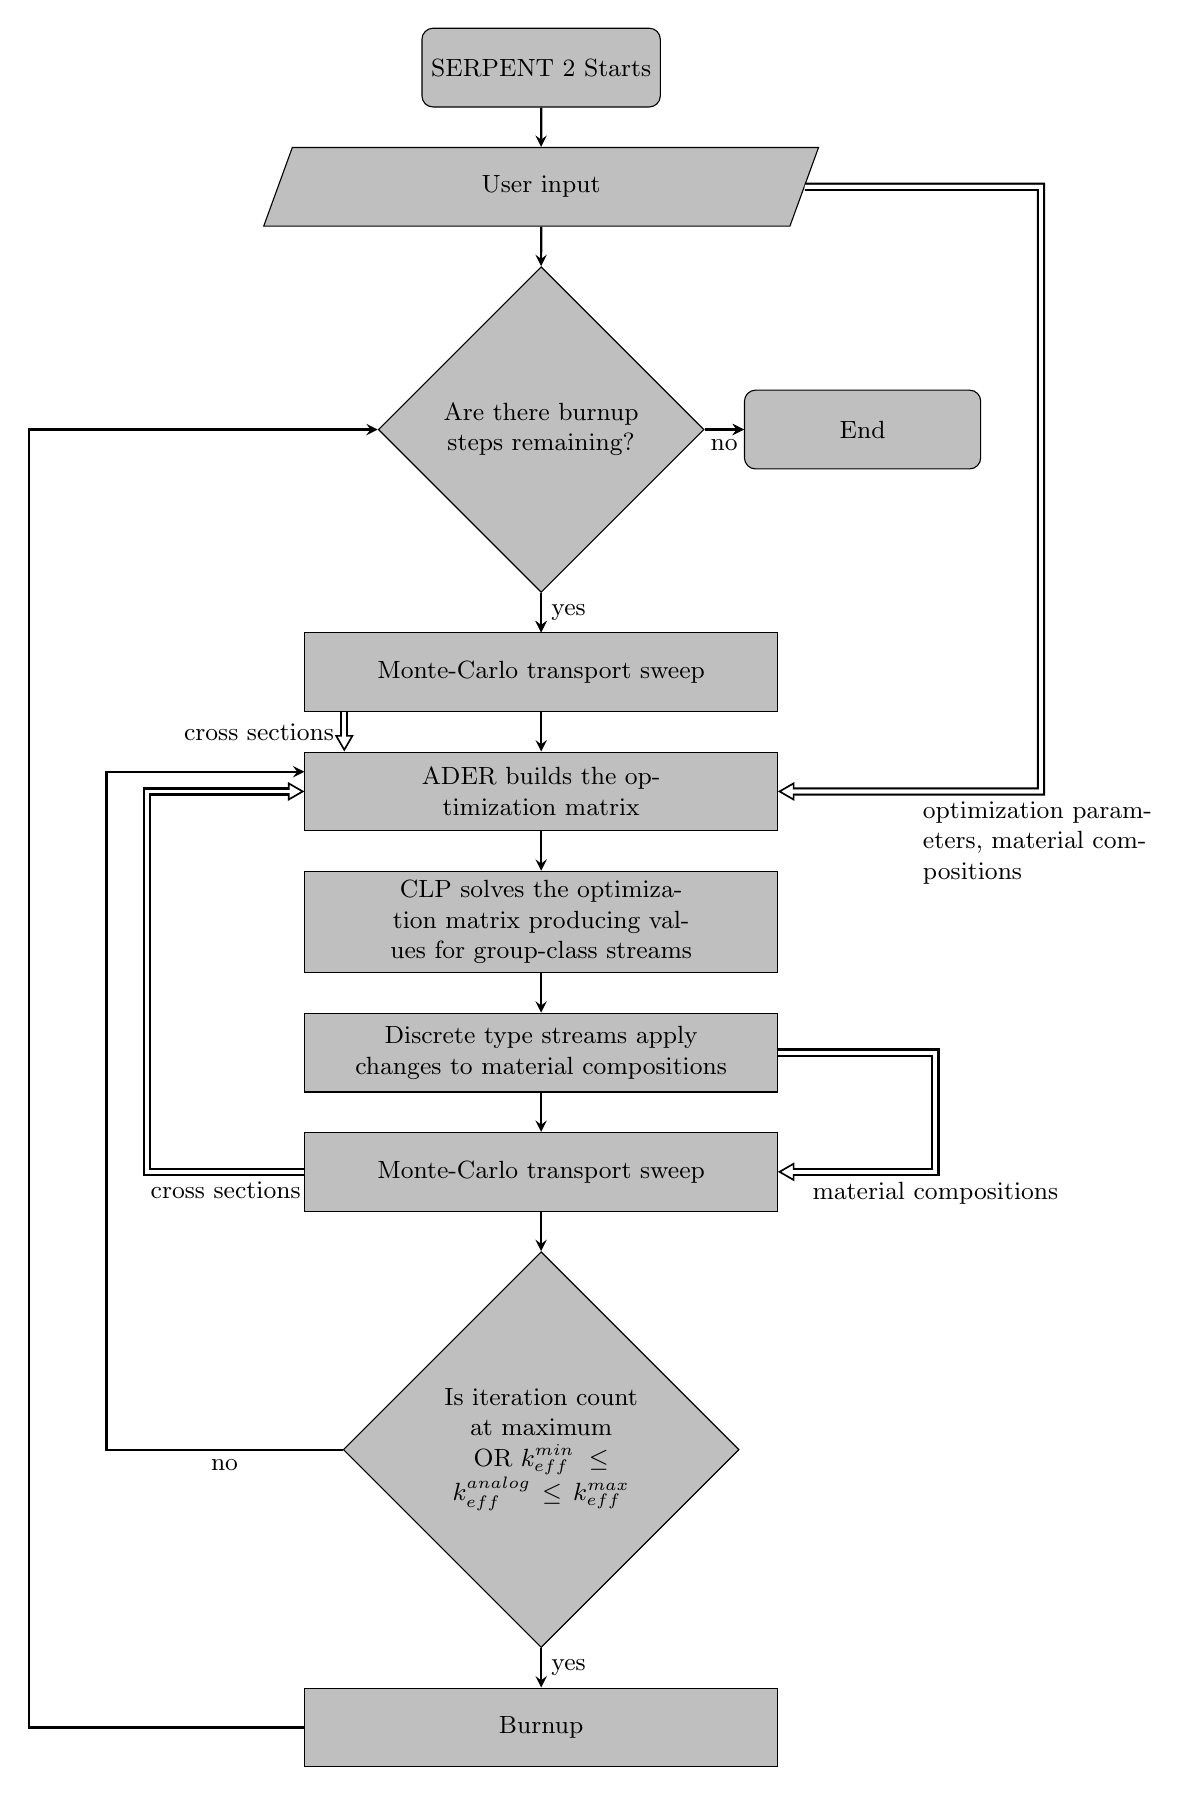
\begin{tikzpicture}[node distance = 1.5cm, every text node part/.style={font=\small}]
\node (start) [startstop] {SERPENT 2 Starts};
\node (input) [io, below=0.5cm of start] {User input};
\node (dec1) [decision, below=0.5cm of input] {Are there burnup steps remaining?};
\node (first) [process, below=0.5cm of dec1] {Monte-Carlo transport sweep};
\node (end) [startstop, right=0.5cm of dec1] {End};
\node (ader_build) [process, below=0.5cm of first] {ADER builds the optimization matrix};
\node (ader_solve) [process, below=0.5cm of ader_build] {CLP solves the optimization
matrix producing values for group-class streams};
\node (ader_apply) [process, below=0.5cm of ader_solve] {Discrete type streams apply changes
to material compositions};
\node (transport) [process, below=0.5cm of ader_apply] {Monte-Carlo transport sweep};
\node (dec2) [decision, below=0.5cm of transport] {Is iteration count at maximum OR $k_{eff}^{min} \leq k_{eff}^{analog} \leq k_{eff}^{max}$};
\node (burn) [process, below=0.5cm of dec2] {Burnup};

\draw [arrow] (start) -- (input);
\draw [arrow] (input) -- (dec1);
\draw [arrow] (dec1) -- (first);
\draw [arrow] (dec1) -- node[anchor=west] {yes} (first);
\draw [arrow] (dec1) -- (end);
\draw [arrow] (dec1) -- node[anchor=north] {no} (end);
\draw [arrow] (first) -- (ader_build);
\draw [vecArrow] (input) -- ([shift={(3cm,0cm)}]input.east) |- node[anchor=north, text width=3cm] {optimization parameters, material compositions} (ader_build.east);
\draw [vecArrow] ([shift={(-2.5cm,0cm)}]first.south) -- node[anchor=east] {cross sections}([shift={(-2.5cm,0cm)}]ader_build.north);
\draw [arrow] (ader_build) -- (ader_solve);
\draw [arrow] (ader_solve) -- (ader_apply);
\draw [vecArrow] (ader_apply) -- ([shift={(2cm,0cm)}]ader_apply.east) |- node[anchor=north] {material compositions} ([shift={(0cm,0cm)}]transport.east);
\draw [arrow] (ader_apply) -- (transport);
\draw [vecArrow] (transport) -- node[anchor=north] {cross sections} ([shift={(-2cm,0cm)}]transport.west) |- ([shift={(0cm,0cm)}]ader_build.west);
\draw [arrow] (transport) -- (dec2);
\draw [arrow] (dec2) -- node[anchor=north] {no} ([shift={(-3cm,0cm)}]dec2.west) |- ([shift={(-1cm,0.25cm)}]ader_build.west) -- ([shift={(0cm,0.25cm)}]ader_build.west);
\draw [arrow] (dec2) -- node[anchor=west] {yes} (burn);
\draw [arrow] (burn) -- ([shift={(-3.5cm,0cm)}]burn.west) |- ([shift={(-3.5cm,0cm)}]dec1.west) -- (dec1);
\end{tikzpicture}
\end{centering}
\caption{A simplified schematic of interactions between SERPENT 2 and ADER. Black lines
represent process flow while double-lined arrows highlight the flow of specific information.}
\end{figure}

\chapter{Test Cases and Results}
\label{sec:results}

This Chapter is Blank

\chapter{Conclusions and Future Work}
\label{ch:conc}

In the last twenty years molten salt reactors have seen an incredible surge of
global attention as evidenced in such international programs as MOSART, ALISIA,
and the LF-TMSR out of China, as well as increased research attention as
evidenced by the continuing success of Oak Ridge National Laboratory's MSR
workshop which now averages over 400 attendees from across the globe yearly. 
While significant investment and progress has been made in nearly all aspects
of MSR development from material selection, salt purification and property
measurement, licensing and general reactor design, comparatively little
attention has been paid to fuel cycle analysis. 

The majority of attempts in
this area have fallen short of producing widely applicable results largely due
to the limiting effects of specific assumptions such as the salt species
involved or the coarseness of the solution. In this work a method and
implementation of a general approach for modelling and evaluating molten salt
reactor fuel cycles is proposed. This approach is based upon a linear
optimization routine designed to approximate the limitations of the chemistry
and nuclear concerns of reactor operations while optimizing the driving concerns
of the reactor operators. This approach, named ADER for the Advanced Depletion
Extension for Reprocessing, is built into the reactor physics Monte-Carlo code
SERPENT 2.  

ADER brings to the users of SERPENT 2 the ability to model several aspects of
MSR operations and fuel cycle analysis through the introduction of several vital
utilities. The first among these is the ability to define collections of
elements, isotopes and chemicals as well as the ability to set absolute and 
relative abundance constraints between any set of these collections, called
groups. In order that ADER might push material compositions towards those which
satisfy the group constraints ADER provides to the user the ability to define
mass transfers into, out of, and between materials in a SERPENT 2 simulation. 
To ensure that these mass transfers do not disturb the desired neutron
multiplication factor in the system ADER allows the user to set neutron 
multiplication maximum and minimum values. During the material optimization
phase ADER estimates the reactivity impact of its selected mass transfers and
adjusts these transfers to keep the system within the desired bounds. Furthermore
ADER provides the ability for the user to set the desired bounds of the averaged
oxidation state of materials in a simulation such that ADER will keep its
selected mass transfers from disturbing the redox potential of the material,
a critical value in determining the effects and extent of corrosive activity. 
Bringing all of this together is an easy to use and directly integrated user
interface supported by a full suite of tests as well as documentation. 

In chapter \ref{ch:results} the results of a simple simulation employing a 
\ce{LiF-BeF2-ThF4-UF4} salt mixture in an infinite and homogeneous medium are
presented. While this simulation did not cause CLP to crash and error out,
nonetheless the results obtained from the simulation present a mixed view of
ADER's implementation. ADER is certainly seen to influence the outcome of the
depletion simulation, adding uranium salts to maintain the minimum value of the
neutron multiplication factor in the system. However, occurring around burnup
step 219, ADER's corrections fail to bring the neutron multiplication value
of the system up to at least the minimum value. ADER did maintain the necessary
amount of fluorine in the system to bind to all primary salt constituents.
However, the mass flows ADER employed to accomplish this took on non-physical
values. With regards to the corrosion monitoring feature of ADER, these
limitations were completely ignored by the simulation for an unknown reason
likely having to do with the inherent numerical instability within the
optimization library. Despite these shortcomings this simulation has undoubtedly
shown the value of an algorithm for incorporating the concerns which ADER
addresses into a nuclear fuel depletion simulation. As put forth in chapter
\ref{ch:method} the implementation of a quad-precision linear optimization solver
should, according to \cite{STANFORD}, resolve the numerical instabilities
plaguing ADER - at which point the algorithm is expected to show great utility
in molten salt reactor analysis.

Any future
work going forth on this project would need to begin with the implementation
of said floating-point quadruple-precision linear optimization solver in the 
place
of the current CLP implementation. Following such a development it is expected
that ADER will be capable of simulating the wide variety of parameters which its
input and structure allow. Additional improvements could be found through the
incorporation of an iteration scheme whereupon the effects of nuclear burnup
on the isotopics of the fuel over a burnup step can be approximated as a
proportional removal stream on the whole system in the linear optimization
scheme such that the approximated total effects of nuclear burnup are considered
in material optimization. 

Overall the impact of ADER is clear in that it represents a more complete
approach to MSR fuel cycle modelling.
Given ADER's extensive test suite, documentation, and modular construction, it
is not unimaginable that the above mentioned improvements may one day be made.
In such a future the impact of ADER would certainly be greater.
Despite this shortcoming ADER has shown that a linear optimization scheme can
be effectively applied to the chemistry, nuclear, and operational concerns of a
molten salt reactor in such a way as to predict the future fuel composition and 
nuclear characteristics of the system.


\bibliographystyle{elsarticle-num}
\bibliography{theory}

\def\StripPrefix#1>{}
\def\jobis#1{FF\fi
  \def\predicate{#1}%
  \edef\predicate{\expandafter\StripPrefix\meaning\predicate}%
  \edef\job{\jobname}%
  \ifx\job\predicate
}

\if\jobis{thesis}
  \bibliography{theory}
\else
  \newpage
  \renewcommand{\thepage}{}
  \bibliography{theory}
\fi

%\appendix
% \include{mathbg}

\end{document}
